\section{\jpc{}, pathwise RL with a jointly trained critic}
\label{sec:method}
Stage 1 uses the trajectory density but leaves its reparameterisability unexploited. Let $V_\phi(y_k)\approx\mathbb E[r\mid y_k,c]$ be a differentiable estimate of success from an intermediate state. Reparameterising one transition as $y_k=\alpha_kD_\theta(y_{k-1})+\sigma_k\varepsilon_k$ yields the pathwise estimator
\begin{equation}
\widehat g_{\mathrm{PW},k}
=
\sum_{i\in\mathcal G}
\frac{\partial V_\phi(y_k)}{\partial y_{k,i}}\,
\alpha_k
\frac{\partial D_\theta(y_{k-1})_i}{\partial\theta}.
\label{eq:pw}
\end{equation}
When $V_\phi$ equals the true value, this is an unbiased estimate of the $k$-th transition's contribution to $\nabla_\theta J$ (Appendix~\ref{app:pw_derivation}). Unlike the score-function estimator in~(\ref{eq:sf}), it replaces the injected-noise factor with the critic's local slope, directly indicating how each state coordinate should change to increase predicted success. The remaining challenge is therefore to learn a critic that accurately scores noisy intermediate states. We develop it in two stages: Stage 2 introduces a scalar critic over flow steps, while Stage 3 extends it across token positions to obtain the \hl{2D critic}. Figure~\ref{fig:mechanism}(b) illustrates the method, and Algorithm~\ref{alg:jpc} summarizes the joint training loop.

\subsection{Stage 2: Scalar critic over flow steps}
\label{sec:jpc_scalar}
We first instantiate \jpc{} with a scalar critic over flow steps. Viewing the flow index as the time step of an MDP, each intermediate state has value $V(y_k,t_k,c)=\mathbb E[r\mid y_k,t_k,c]$ under the current policy. This value requires no intermediate supervision: we retain several states from each rollout and train $V_\phi$ against their shared terminal outcome using binary cross-entropy (BCE). The critic reuses a copy of the denoiser trunk to produce per-position features $f_i(y_k,t_k,c)$, pools them over generated positions, and applies a scalar head,
\[
V_\phi(y_k,t_k,c)=h_\phi\bigl(\frac{1}{|\mathcal G|}\sum_{i\in\mathcal G}f_i(y_k,t_k,c),t_k\bigr).
\]
The policy then ascends this value through the pathwise update in~(\ref{eq:pw}). Pooling before value estimation removes the token-position axis: the critic can identify whether an intermediate state is promising, but not which positions are responsible, which motivates 2D critic in the next section.

\subsection{Stage 3: 2D critic over flow steps and token positions}
\label{sec:jpc_2d}

AR generation has one natural credit-assignment axis: the RL time step coincides with token position. Actions $w_t$, advantages $A_t$, PPO ratios $\rho_t$, and prefix values $V(w_{<t})$ are all indexed by $t$; credit assignment is therefore one-dimensional, operating solely along the sequence. A flow language model instead generates a grid of states $y_{k,i}$ over flow steps $k$ and token positions $i$, with all positions refined jointly throughout the trajectory. Existing flow RL methods \citep{liu2025flowgrpo, xue2025dancegrpo} and scalar JPC retain only the flow-step axis: the former assign sequence-level credit to denoising steps, while the latter pool position features before estimating value at each flow step. This discards the token-position axis on which semantic decisions are represented, motivating a critic indexed by both \emph{when} along the flow and \emph{where} along the sequence.

To restore the token-position axis, we replace the scalar critic's pool-then-head architecture with a head-then-pool architecture. Given the per-position features $f_i(y_k,t_k,c)$, the 2D critic produces
\begin{equation}
R_{\phi,k,i}
=
h_\phi\bigl(f_i(y_k,t_k,c),t_k\bigr),
\qquad
V_\phi(y_k,t_k,c)
=
\frac{1}{|\mathcal G|}
\sum_{i\in\mathcal G}R_{\phi,k,i}.
\label{eq:critic2d}
\end{equation}
The resulting value field is indexed by both flow step $k$, specifying \emph{when} the state is evaluated, and token position $i$, specifying \emph{where} credit is assigned. The actor still ascends the pooled value $V_\phi$ through~(\ref{eq:pw}), but each state position now receives a direct gradient through its own nonlinear head rather than only through a pooled bottleneck. The critic requires no token-level labels. We supervise both its pooled value and its per-position field using the same terminal outcome:
\begin{equation}
\mathcal L_{\mathrm{2D}}(\phi)
=
\frac{1}{2}\,
\mathrm{BCE}\!\left(\sigma(V_\phi),r\right)
+
\frac{1}{2|\mathcal G|}
\sum_{i\in\mathcal G}
\mathrm{BCE}\!\left(\sigma(R_{\phi,k,i}),r\right).
\label{eq:critic2d_loss}
\end{equation}
The position-wise term does not provide local correctness labels; rather, it prevents the field from collapsing into an uninformative pooled representation while preserving supervision from sequence-level verifier outcomes.


\begin{algorithm}[t]
\caption{\jpc{}-2D training}
\label{alg:jpc}
\small
\begin{algorithmic}[1]
\REQUIRE policy $D_\theta$; pre-trained critic $V_\phi$; verifier $r$; prompt set $\mathcal C$; update-step window $\mathcal W$; number of updates $T$; critic steps per iteration $m$; replay buffer $\mathcal B$; buffer size $N$; rollout steps $K$; batch size $B$; minibatch size $B'$; learning rates $\eta_\theta,\eta_\phi$
\FOR{iteration $=1,\dots,T$}
  \STATE Sample a batch of prompts $c=\{c^j\}_{j=1}^B \sim \mathcal C$ and a flow step $k\sim\mathcal U(\mathcal W)$
  \STATE Rollout $\{(y_0, \dots, y_{k-1})^j\}_{j=1}^B$ without gradients up to $k-1$
  \STATE Compute $y_k^j=\alpha_kD_\theta(y_{k-1}^j)+\sigma_k\varepsilon_k^j,\;\varepsilon_k^j\sim\mathcal N(0,I)$ with gradients, keeping $V_\phi$ fixed
  \STATE \textbf{Update the policy:}  $\theta\leftarrow\theta+\eta_\theta\nabla_\theta E_B [V_\phi(y_k)]$
  \STATE Sample a fresh batch of prompts $c'=\{c'^j\}_{j=1}^B \sim \mathcal C$ 
  \STATE Rollout full K steps $\{(y_0, \dots, y_K)^j\}_{j=1}^B$ from updated policy without gradients
  \STATE Compute the verifier outcomes $r=\{r(\text{decode}(y_K^j),c'^j)\}_{j=1}^B$
  \STATE $\mathcal B \leftarrow \mathcal B \cup \{(y_{k'},k',c',r)^j\}_{j=1}^B$ for $\{k'\} \sim \mathcal W$ and keep the newest $N$ states 
  \FOR{inner iteration $=1,\dots,m$}
    \STATE Sample a minibatch of states $\{(y_{k'},k',c',r)^j\}_{j=1}^{B'} \sim \mathcal B$
    \STATE \textbf{Update the critic:} $\phi\leftarrow\phi-\eta_\phi\nabla_\phi E_{B'}[ \mathrm{BCE}(\sigma(V_\phi(y_{k'})),r)]$
  \ENDFOR
\ENDFOR
\end{algorithmic}
\end{algorithm}

\begin{figure}[t]
\centering
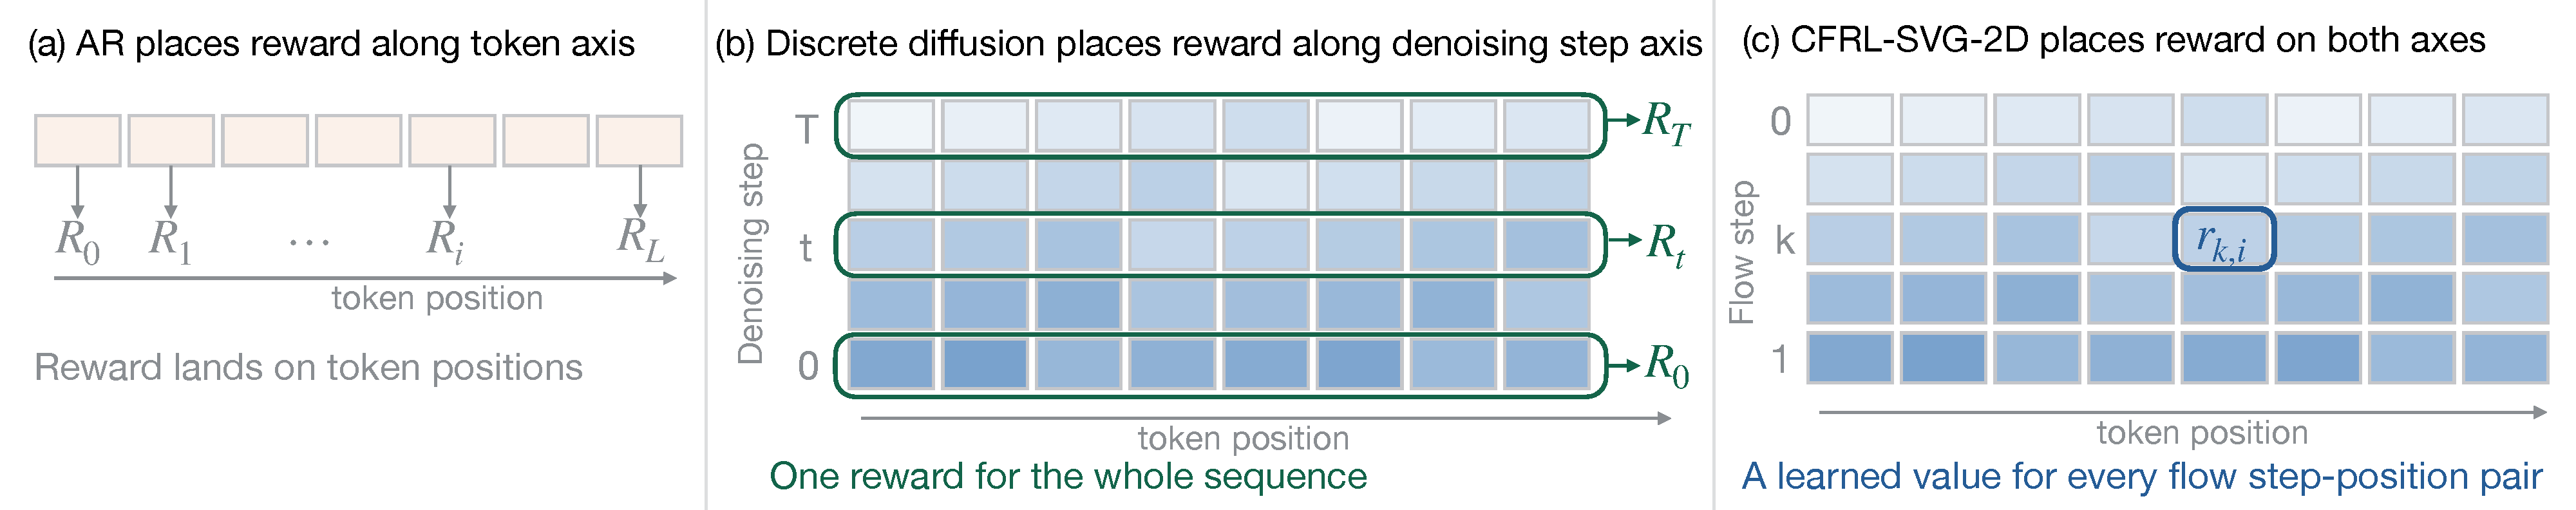
\includegraphics[width=0.78\linewidth]{figures/flow-rl-figure1.pdf}
\caption{(a) RL on AR models assigns reward over token positions (b) RL on discrete diffusions assigns reward over flow steps (c) \jpc{}-2D critic places reward on both flow steps and token positions.}
\label{fig:mechanism}
\end{figure}


